%  LaTeX support: latex@mdpi.com 
%  For support, please attach all files needed for compiling as well as the log file, and specify your operating system, LaTeX version, and LaTeX editor.

%=================================================================
\documentclass[sensors,article,submit,pdftex,moreauthors]{Definitions/mdpi} 
% For posting an early version of this manuscript as a preprint, you may use "preprints" as the journal and change "submit" to "accept". The document class line would be, e.g., \documentclass[preprints,article,accept,moreauthors,pdftex]{mdpi}. This is especially recommended for submission to arXiv, where line numbers should be removed before posting. For preprints.org, the editorial staff will make this change immediately prior to posting.

%--------------------
% Class Options:
%--------------------
%----------
% submit
%----------
% The class option "submit" will be changed to "accept" by the Editorial Office when the paper is accepted. This will only make changes to the frontpage (e.g., the logo of the journal will get visible), the headings, and the copyright information. Also, line numbering will be removed. Journal info and pagination for accepted papers will also be assigned by the Editorial Office.

%------------------
% moreauthors
%------------------
% If there is only one author the class option oneauthor should be used. Otherwise use the class option moreauthors.

%---------
% pdftex
%---------
% The option pdftex is for use with pdfLaTeX. If eps figures are used, remove the option pdftex and use LaTeX and dvi2pdf.

%=================================================================
% MDPI internal commands
\firstpage{1} 
\makeatletter 
\setcounter{page}{\@firstpage} 
\makeatother
\pubvolume{1}
\issuenum{1}
\articlenumber{0}
\pubyear{2022}
\copyrightyear{2022}
%\externaleditor{Academic Editor: Firstname Lastname}
\datereceived{} 
\dateaccepted{} 
\datepublished{} 
%\datecorrected{} % Corrected papers include a "Corrected: XXX" date in the original paper.
%\dateretracted{} % Corrected papers include a "Retracted: XXX" date in the original paper.
\hreflink{https://doi.org/} % If needed use \linebreak
%\doinum{}
%------------------------------------------------------------------
% The following line should be uncommented if the LaTeX file is uploaded to arXiv.org
%\pdfoutput=1

%=================================================================
% Add packages and commands here. The following packages are loaded in our class file: fontenc, inputenc, calc, indentfirst, fancyhdr, graphicx, epstopdf, lastpage, ifthen, lineno, float, amsmath, setspace, enumitem, mathpazo, booktabs, titlesec, etoolbox, tabto, xcolor, soul, multirow, microtype, tikz, totcount, changepage, attrib, upgreek, cleveref, amsthm, hyphenat, natbib, hyperref, footmisc, url, geometry, newfloat, caption

%=================================================================
%% Please use the following mathematics environments: Theorem, Lemma, Corollary, Proposition, Characterization, Property, Problem, Example, ExamplesandDefinitions, Hypothesis, Remark, Definition, Notation, Assumption
%% For proofs, please use the proof environment (the amsthm package is loaded by the MDPI class).

%=================================================================
% Full title of the paper (Capitalized)
\Title{A Deep Learning Approach for Gait Event Detection from a Single Shank-Worn IMU: Validation in Healthy and Neurological Cohorts}

% MDPI internal command: Title for citation in the left column
\TitleCitation{A Deep Learning Approach for Gait Event Detection from a Single Shank-Worn IMU: Validation in Healthy and Neurological Cohorts}

% Author Orchid ID: enter ID or remove command
\newcommand{\orcidauthorA}{0000-0002-2507-0924} % Add \orcidA{} behind the author's name
%\newcommand{\orcidauthorB}{0000-0000-0000-000X} % Add \orcidB{} behind the author's name

% Authors, for the paper (add full first names)
\Author{Robbin Romijnders$^{1}$*\orcidA{}, Elke Warmerdam$^{2}$, Clint Hansen$^{1}$, Gerhard Schmidt$^{3}$ and Walter Maetzler$^{1}$}

%\longauthorlist{yes}

% MDPI internal command: Authors, for metadata in PDF
\AuthorNames{Robbin Romijnders, Elke Warmerdam, Clint Hansen, Gerhard Schmidt and Walter Maetzler}

% MDPI internal command: Authors, for citation in the left column
\AuthorCitation{Romijnders, R.; Warmerdam, E.; Hansen, C.; Schmidt, G.; Maetzler, W.}
% If this is a Chicago style journal: Lastname, Firstname, Firstname Lastname, and Firstname Lastname.

% Affiliations / Addresses (Add [1] after \address if there is only one affiliation.)
\address{%
$^{1}$ \quad Department of Neurology, Kiel University, 24105 Kiel, Germany; r.romijnders@neurologie.uni-kiel.de (R.R.), c.hansen@neurologie.uni-kiel.de (C.H.), w.maetzler@neurologie.uni-kiel.de (W.M.)\\
$^{2}$ \quad Innovative Implant Development (Fracture Healing), Division of Surgery, Saarland University, 66421 Homburg, Germany; elke.warmerdam@uni-saarland.de (E.W.)\\
$^{3}$ \quad Institute of Electrical Engineering and Information Technology, Faculty of Engineering, Kiel University, 24143 Kiel, Germany; gus@tf.uni-kiel.de (G.S.)}

% Contact information of the corresponding author
\corres{Correspondence: r.romijnders@neurologie.uni-kiel.de (R.R.)}

% Current address and/or shared authorship
%\firstnote{Current address: Affiliation 3.} 
%\secondnote{These authors contributed equally to this work.}
% The commands \thirdnote{} till \eighthnote{} are available for further notes

%\simplesumm{} % Simple summary

%\conference{} % An extended version of a conference paper

% Abstract (Do not insert blank lines, i.e. \\) 
\abstract{Many algorithms use 3D accelerometer and/or gyroscope data from inertial measurement unit (IMU) sensors to detect gait events (i.e., initial and final foot contact). However, these algorithms often require knowledge about sensor orientation and use empirically derived thresholds. As sensor-to-segment alignment cannot always be controlled for in ambulatory assessments, methods are needed that require little knowledge on sensor location and orientation, e.g., a convolutional neural network-based deep learning model. Therefore, 160 participants from healthy and neurologically diseased cohorts walked 5 meter distances at slow, preferred, and fast walking speed, while data were collected from IMUs on the left and right ankle and shank. Gait events were detected and stride parameters were extracted using a deep learning model and an optoelectronic motion capture (OMC) system for reference. Results showed a high detection rate for both initial and final contacts across sensor locations (recall $\ge 92\%$, precision $\ge 97\%$). Time agreement was excellent as witnessed from the median time error (0.005 s) and corresponding inter-quartile range (0.020 s). The extracted stride-specific parameters were in good agreement with parameters derived from the OMC system (maximum mean difference 0.003 s, and corresponding maximum limits of agreement (-0.049 s, 0.051 s) for a $95\%$ confidence level.) Thus, the deep learning approach was considered a valid approach for detecting gait events and extracting stride-specific parameters with little knowledge on exact IMU location and orientation in conditions with and without walking pathologies due to neurological diseases.}

% Keywords
\keyword{gait; gait events; interial measurement unit; deep learning} 

% The fields PACS, MSC, and JEL may be left empty or commented out if not applicable
%\PACS{J0101}
%\MSC{}
%\JEL{}

%%%%%%%%%%%%%%%%%%%%%%%%%%%%%%%%%%%%%%%%%%
% Only for the journal Diversity
%\LSID{\url{http://}}

%%%%%%%%%%%%%%%%%%%%%%%%%%%%%%%%%%%%%%%%%%
% Only for the journal Applied Sciences:
%\featuredapplication{Authors are encouraged to provide a concise description of the specific application or a potential application of the work. This section is not mandatory.}
%%%%%%%%%%%%%%%%%%%%%%%%%%%%%%%%%%%%%%%%%%

%%%%%%%%%%%%%%%%%%%%%%%%%%%%%%%%%%%%%%%%%%
% Only for the journal Data:
%\dataset{DOI number or link to the deposited data set in cases where the data set is published or set to be published separately. If the data set is submitted and will be published as a supplement to this paper in the journal Data, this field will be filled by the editors of the journal. In this case, please make sure to submit the data set as a supplement when entering your manuscript into our manuscript editorial system.}

%\datasetlicense{license under which the data set is made available (CC0, CC-BY, CC-BY-SA, CC-BY-NC, etc.)}

%%%%%%%%%%%%%%%%%%%%%%%%%%%%%%%%%%%%%%%%%%
% Only for the journal Toxins
%\keycontribution{The breakthroughs or highlights of the manuscript. Authors can write one or two sentences to describe the most important part of the paper.}

%%%%%%%%%%%%%%%%%%%%%%%%%%%%%%%%%%%%%%%%%%
% Only for the journal Encyclopedia
%\encyclopediadef{Instead of the abstract}
%\entrylink{The Link to this entry published on the encyclopedia platform.}
%%%%%%%%%%%%%%%%%%%%%%%%%%%%%%%%%%%%%%%%%%
\begin{document}

%%%%%%%%%%%%%%%%%%%%%%%%%%%%%%%%%%%%%%%%%%
\section{Introduction}
Gait deficits are common in older adults and possibly reflect the presence of an underlying neurodegenerative disease \cite{Snijders2007,Hodgins2008}. For example, conversion to Parkinson's Disease \cite{DelDin2019} or conversion from mild cognitive impairment to Alzheimer's Disease \cite{Koenig2017,Bertoli2018} are linked with changes in spatiotemporal gait parameters. Similarly, temporal gait parameters are different for stroke patients \cite{SchroederVon1995,Mohan2021} and patients with multiple sclerosis \cite{Griskevicius2016,Flachenecker2019} when compared to healthy controls. To objectively quantify gait deficits, stride-specific parameters such as stride time or stride length are often used \cite{Hannink2016}. The beginning and end of a stride are determined from two successive initial contacts (ICs) of the same foot \cite{Perry2010,Whittle2012}. The IC is when the foot contacts the ground and together with the instant at which the foot leaves the ground (final contact, FC), each stride can be divided in a stance and swing phase \cite{Rueterbories2010,Bruening2014}.  The events of IC and FC, also referred to as \emph{gait events}, are commonly determined using force or pressure measuring devices \cite{Bruening2014}, or marker-based optoelectronic motion capture systems (henceforth referred to as the \emph{marker-based} system or method) \cite{Chiari2005,Topley2020}. These systems are relatively expensive, and restricted to usage in expertise laboratories \cite{Iosa2016,Jarchi2018}. As there is increasing evidence that gait measured in the lab does not reflect daily-life gait \cite{Hillel2019,Warmerdam2020,Atrsaei2021}, there is increasingly more interest in measurement systems that allow for continuous gait analysis in ambulatory settings. Therefore, the use of inertial measurement units (IMUs) is especially attractive, as these can be used to measure gait in ecologically valid environments, such as the home environment, thereby painting a more complete picture of health status \cite{DelDin2016,Shah2020} and providing clinical information that is complementary to standardized lab-based assessments \cite{Warmerdam2020,Fasano2020,Atrsaei2021,Corra2021}.

Previous research suggests that gait event detection is more accurate using an IMU worn on a lower limb (e.g., shank or foot) compared to an IMU worn on the low back \cite{BenMansour2015,Storm2016,Panebianco2018}. Now, in order to get from abstract IMU sensor readings to clinically relevant gait parameters (e.g., from accelerations and angular velocities to stride times) \cite{Hannink2016}, different algorithmic approaches have been developed in the last twenty years of clinical gait research. A recent study has evaluated a cross-section of these algorithms for different sensor locations on the lower leg and foot \cite{Niswander2021}. The algorithms were categorized according to which signals were analyzed, for example the angular velocity about the medio-lateral axis, or the accelerations along vertical and antero-posterior axes. This means the sensor readings need to be linked with the anatomical axes, that is, one needs to know which sensor axis aligns with for example the medio-lateral axis. In most approaches, it is simply assumed that due to sensor attachment the sensor axis aligns roughly with the anatomical axis of interest (\cite{Salarian2004,Sabatini2005,Jasiewicz2006,Catalfamo2010,Trojaniello2014,Maqbool2016,Romijnders2021}) or an additional calibration procedure (e.g., \cite{Ferraris1995}) is required (\cite{Greene2010,Niswander2021}). In ambulatory assessments however, study participants often attach the sensor themselves, for example after showering, and therefore the sensor location and alignment cannot be controlled for. Furthermore, it is unlikely that each time the sensor is (re-)attached study participants, especially those with gait deficits, perform a calibration procedure that usually consists of holding a pre-defined pose and performing some known movement sequences \cite{Leineweber2019,Pacher2020}. 

Taken together, this drives the need for an approach that is invariant to sensor orientation, and is applicable across a variety of pathological gait patterns. In the field of image analysis similar requirements have been successfully addressed by algorithms that share a common underlying methodology referred to as deep learning \cite{LeCun2015,Hannink2016,TerHaarRomeny2019}. Recent applications of deep learning algorithms have already shown improved performance in detecting gait events from marker-based motion capture when compared to conventional, often heuristics-based, algorithms \cite{Kidzinski2019,Lempereur2020,Filtjens2020}. Another study used a deep learning approach to detect gait events from either three IMUs (worn on the low back, and both ankles) or a single IMU (worn on the low back), and showed that the time error was considerably smaller for the deep learning algorithm than for a commonly applied wavelet-based approach \cite{Gadaleta2019}.

The aim of this study is to extend these works by validating this deep learning approach for detecting gait events in a heterogeneous cohort of healthy and neurologically diseased adults considering a single IMU setup, worn on the lower leg.
%%%%%%%%%%%%%%%%%%%%%%%%%%%%%%%%%%%%%%%%%%
\section{Materials and Methods}
\subsection{Data Collection}
Gait analyses were performed in the Universit\"{a}tsklinikum Schleswig-Holstein (UKSH) campus Kiel, Germany. The study \cite{Warmerdam2021} was approved by the ethical committee of the medical faculty at the UKSH (no: D438/18). In total, data from 160 participants were included for the current analysis, including data from young adults (YA; age: 18 - 60 years), older adults (OA; age: $>$60 years), people with Parkinson's Disease (PD; according to the UK Brain Bank criteria \cite{Gibb1988}), people with a recent ($<$4 weeks) symptomatic stroke (stroke), people with multiple sclerosis (MS; according to the McDonalds criteria \cite{Thompson2018}), people with chronic low back pain (cLBP), and people with diagnoses not fitting in any before-mentioned groups or disorders with no explicit diagnosis (other) (Table \ref{tab:demographics_data}). Inclusion criteria were an age of 18 years or older, and the ability to walk independently without a walking aid. Participants were excluded from the study with a Montreal Cognitive Assessment \cite{Nasreddine2005} score $<$15 and other movement disorders that affected mobility, as noticed by the clinical assessor.

\begin{table}[H] 
	\caption{\label{tab:demographics_data}Demographics data of the study participants. Age, height, and weight are presented as mean (standard deviation).}
	\newcolumntype{C}{>{\centering\arraybackslash}X}
	\begin{tabularx}{\textwidth}{CCCCCC}
		\toprule
		\textbf{Group}	& \textbf{Gender}	& \textbf{Number of}	& \textbf{Age}	& \textbf{Height}	& \textbf{Weight}\\
		 & & \textbf{participants} & years	& cm	& kg\\
		\midrule
		YA		& F		& 21	& 27 (7)	& 173 (5)	& 67 (8)\\
		 & M	& 22	& 30 (9)	& 185 (8) & 81 (13)\\ 
		\midrule
		OA		& F		& 11	& 70 (6)	& 167 (6)	& 72 (17)\\
		 & M	& 11	& 73 (6)	& 180 (6) & 83 (11)\\
		\midrule
		PD		& F		& 12	& 67 (6)	& 168 (6)	& 70 (14)\\
		 & M	& 20	& 62 (11)	& 178 (6) & 87 (13)\\
		\midrule
		MS		& F		& 12	& 37 (9)	& 174 (9)	& 75 (9)\\
		 & M	& 9	& 42 (15)	& 189 (8) & 96 (30)\\
		\midrule
		stroke	& F		& 4	& 66 (10)	& 160 (6)	& 65 (11)\\
		 & M	& 17	& 67 (17)	& 178 (7) & 84 (14)\\
		\midrule
		cLBP	& F		& 3	& 64 (10)	& 166 (5)	& 65 (5)\\
		 & M	& 7	& 63 (16)	& 178 (7) & 90 (16)\\ 
		\midrule
		other	& F		& 3	& 60 (13)	& 166 (3)	& 79 (15)\\
		 & M	& 8	& 68 (18)	& 182 (7) & 85 (13)\\ 
		\bottomrule
	\end{tabularx}
	\noindent{\footnotesize{\textbf{Group}: YA: younger adults, OA: older adults, PD: Parkinson's Disease, MS: multiple sclerosis, cLBP: chronic low back pain; \textbf{Gender}: F: female, M: male.}}
\end{table}

\begin{figure}[H]
	\begin{adjustwidth}{-\extralength}{0cm}
		\centering
		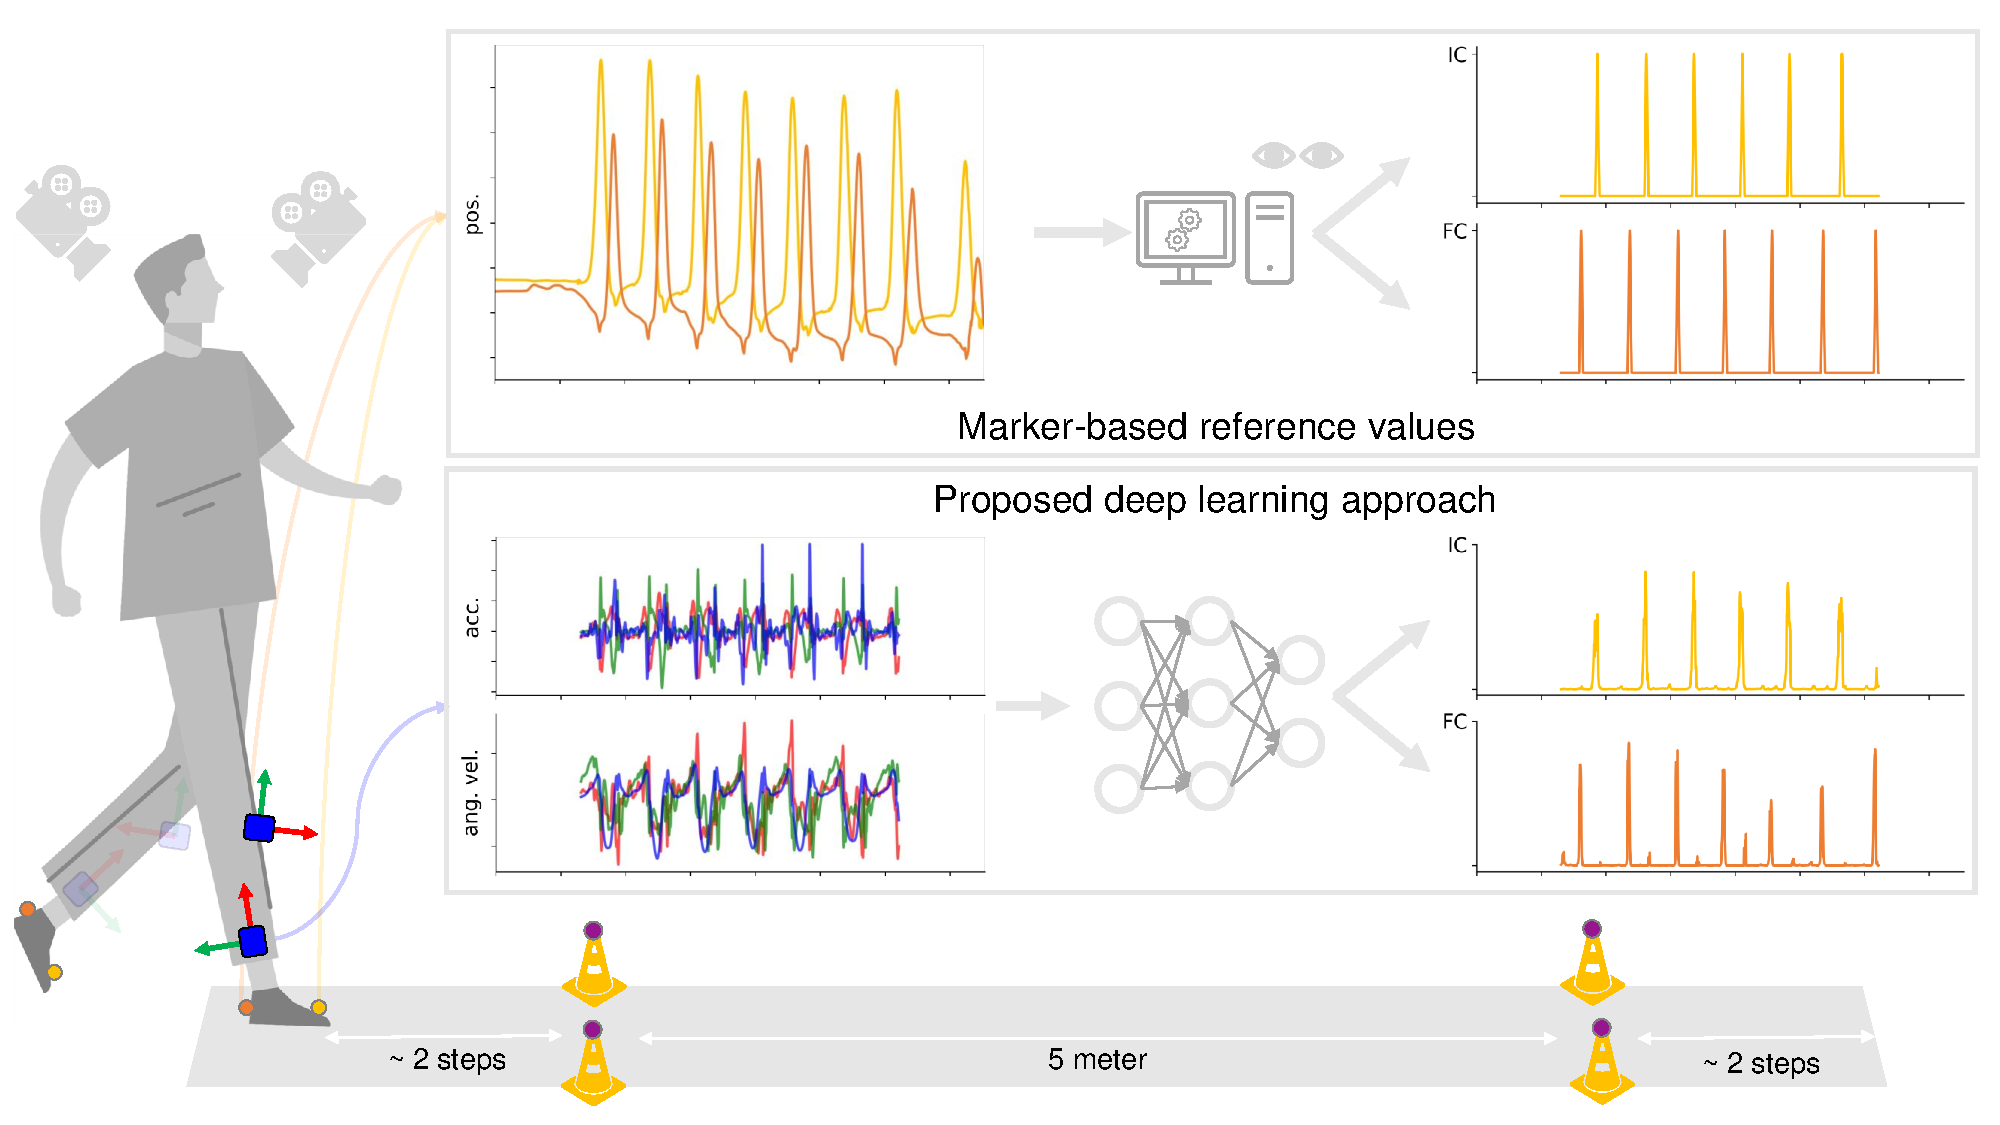
\includegraphics[width=13.5cm]{fig/methods_overall_workflow.pdf}
	\end{adjustwidth}
	\caption{Schematic depiction$^{1}$ of the current study. Study participants wore IMUs on the ankle and shanks, and reflective markers were adhered on the heel and toe of usual footwear (illustrated on the left). Marker data were used to obtain reference values for the timings of initial and final contacts (top), where accelerometer and gyroscope data from each tracked point were inputted to a neural network that predicted timings of the same initial and final contacts (bottom). \newline \noindent{\footnotesize{\textsuperscript{1} Picture from: \url{https://www.vecteezy.com/free-vector/man-walking }.}} \label{fig:methods_marker_vs_imu}}
\end{figure}  

Participants performed three walking trials consisting of walking 5 meter at either (1) preferred speed ("\emph{Please walk at your normal walking speed.}"), (2) slow speed ("\emph{Please walk at half of your normal walking speed.}"), or (3) fast speed ("\emph{Please walk as fast as possible, without running or falling.}"). The 5 meter distance was marked with two cones on both ends, and participants were asked to start walking approximately two steps before the cones on one end, and stop walking approximately two steps after passing the cones on the other end.

For the current analysis data from four IMUs (Noraxon USA Inc., myoMOTION, Scottsdale, AZ, USA) were considered, namely those that were attached laterally above the left and right ankle joint and those attached proximally at the left and right shank. IMUs were secured to participants using elastic bands with a special hold for the IMU. Furthermore, reflective markers were attached on top of the usual foot wear at the heel and toe of both feet (Figure~\ref{fig:methods_marker_vs_imu}). Marker data were recorded using a twelve-camera optoelectronic motion capture system (Qualisys AB, G\"{o}teborg, Sweden) at a sampling frequency of 200 Hz. IMU data were recorded at the same sampling frequency, and both systems were synchronized using a TTL signal \cite{Warmerdam2021}.

\subsection{Data Pre-processing \label{subsec:data_preprocessing}}
\subsubsection{Marker Data}
First, data from both marker and IMU systems were cropped so that only data from within the 5 meter distance were considered. Any gaps in the marker data were filled by interpolation making use of inter-correlations between markers \cite{Federolf2013,Gloersen2016}. The data were then low-pass filtered using a 6th order Butterworth filter with a cut-off frequency of 20 Hz \cite{Racz2021}. The filter was applied twice to the input data \cite{Kormylo1974}. After filtering in forward direction, the filtered sequence was reversed and run back through the filter \cite{Salarian2004}. The filtered data were differentiated to get velocity signals, and timings of ICs and FCs were determined from local maxima and minima in the heel and toe vertical velocity signals \cite{Pijnappels2001,OConnor2007}. All identified ICs and FCs were manually checked using Qualisys Track Manager 2018.1 software (Qualisys AB, Göteborg, Sweden), and corrected if necessary \cite{Carcreff2018,Romijnders2021}. The resulting annotated ICs and FCs were considered the \emph{true} events (also \emph{labels} or \emph{targets}), and were used as reference timings to derive stride-specific gait parameters.

\subsubsection{IMU Data}
The idea behind the deep learning approach was that a \emph{model} was trained to predict the likelihood of an IC and FC, given accelerometer and gyroscope data from a single IMU. The data from a single sensor channel, e.g., the acceleration in forward direction, was denoted by $\mathbf{x}_{d} = \begin{bmatrix}
	x_{d}[1] & x_{d}[2] & \cdots & x_{d}[N]
\end{bmatrix}^{\mathrm{T}}$, with $d$ referring to the $d$th sensor channel (i.e., $d = 1, \cdots, D$) and $n$ referring to the $n$th sample or time step (i.e., $n = 1, \cdots, N$). Similarly, the data from all $D$ sensor channels at a given time instant $n$, was denoted by $\mathbf{x}[n] = \begin{bmatrix}
x_{1}[n] & x_{2}[n] & \cdots & x_{D}[n]
\end{bmatrix}^{\mathrm{T}}$. Data from all $D$ channels, and for all $N$ time steps, was then denoted by:
\begin{equation}
	\mathbf{X} = \begin{bmatrix}
		\rule[0ex]{0.5pt}{2.5ex} & \rule[0ex]{0.5pt}{2.5ex} &  & \rule[0ex]{0.5pt}{2.5ex}\\
		\mathbf{x}_{1} & \mathbf{x}_{2} & \cdots & \mathbf{x}_{D}\\
		\rule[0ex]{0.5pt}{2.5ex} & \rule[0ex]{0.5pt}{2.5ex} &  & \rule[0ex]{0.5pt}{2.5ex}
	\end{bmatrix} = \begin{bmatrix}
		x_{1}[1] & x_{2}[1] & & x_{D}[1]\\
		x_{1}[2] & x_{2}[2] & & x_{D}[2]\\
		\vdots & \vdots & \cdots & \vdots\\
		x_{1}[N] & x_{2}[N] & & x_{D}[N]\end{bmatrix}, \quad \mathbf{X} \in \mathbb{R}^{N \times D}
	\label{eqn:train_data_single_instance}
\end{equation}

Likewise, the \emph{labels} were denoted by:
\begin{equation}
	\mathbf{y}_{\mathrm{IC}} = \begin{bmatrix}
		y_{\mathrm{IC}}[1]\\
		y_{\mathrm{IC}}[2]\\
		\vdots\\
		y_{\mathrm{IC}}[N]
	\end{bmatrix}, \quad \mathbf{y}_{\mathrm{FC}} = \begin{bmatrix}
		y_{\mathrm{FC}}[1]\\
		y_{\mathrm{FC}}[2]\\
		\vdots\\
		y_{\mathrm{FC}}[N]
	\end{bmatrix}, \quad y_{\mathrm{IC}/\mathrm{FC}}[n] \in [0, 1]
	\label{eqn:train_labels_single_instace}
\end{equation}

The model was iteratively trained to learn a mapping $h_{\mathbf{\Theta}}(\mathbf{X}): \mathbf{X} \rightarrow \mathbf{y}$, where $h_{\mathbf{\Theta}}$ was also referred to as the \emph{hypothesis} parameterized by the weights, collectively denoted by $\mathbf{\Theta}$.

All participant data data were split in three independent data sets, namely a training set, a validation set, and a test set. Each set contained data from approximately one-third of the participants. Participants were randomly assigned to one of the sets, stratified by both group (i.e., diagnosis) and gender (Table~\ref{tab:demographics_data}). The training and validation set were used to train an optimal deep learning model. Test set data were not used for model training or hyperparameter tuning. The results on the model's performance were only based on the test set, and therefore reflect how good the model generalizes to new, \emph{unseen} data.

Accelerometer and gyroscope data were normalized by subtracting the channel-wise mean, and dividing by the channel-wise standard deviation. Then, for the training and validation data set, the data were partitioned into equal length time windows \cite{Filtjens2020} of 400~samples, with an overlap of 50\% between successive windows (corresponding to 2 s windows, and 1 s overlap, respectively).

\subsection{Model}
\subsubsection{Model Architecture}
The generic architecture for the deep learning model was based on a temporal convolutional network (TCN) \cite{Bai2018,Remy2020,Filtjens2020}. The TCN consisted of a sequence of residual blocks with exponentially increasing dilation factor \cite{YuKoltun2016,Bai2018}. Each residual block was built from two sequences of a dilated convolutional layer \cite{YuKoltun2016}, a batch normalization layer \cite{Ioffe2015}, a rectified linear unit (ReLU) activation layer, and a dropout layer \cite{Srivastava2014} (Figure). The model was built in Python \cite{VanRossum2009} using the high-level TensorFlow API Keras \cite{Remy2020,Chollet2015}.

For the current analysis only convolutions of the "same" type were considered \cite{Remy2020}, i.e., the model was non-causal and zero-padded to account for edge effects, and the likelihood of an IC or FC was based on input data both before and after the current sample, $n$:
\begin{equation}
	\hat{y}_{i}[n] = f\left(\cdots, \mathbf{x}[n-1], \mathbf{x}[n], \mathbf{x}[n+1], \cdots \right), \quad i \in \left\{ \mathrm{IC}, \mathrm{FC}\right\}
\end{equation}
The number of samples that the predictions at time $n$ "sees", was referred to as the \emph{receptive field} \cite{Lea2017} and was a function of the kernel size and the dilation factors \cite{Remy2020}. Dilation factors were always given as a sequence of increasing power of 2 \cite{YuKoltun2016,Bai2018,VanDenOord2016}.

The outputs of the TCN block were fed to two separate fully-connected (FCN, or dense) layers, that both were followed by a sigmoid activation layer. Outputs were then predicted separately for ICs and FCs \cite{Gadaleta2019,Filtjens2020}. The mean squared error (MSE) was used as a loss function, and a gradient descent-based optimization algorithm with adaptive moment (Adam) optimizer was used to iteratively learn the weights \cite{Kingma2014,Schmidt2021}.

\subsubsection{Hyperparameter Optimization}
In order to find the best model architecture, hyperparameter tuning was perfomed using KerasTuner \cite{OMalley2019}. Here, the number of filters, the kernel size, and the maximum dilation factor (Table \ref{tab:hyperparameter_optimization}) were optimized for using a random search strategy \cite{Bergstra2012}.

\begin{table}[H] 
	\caption{Model hyperparameters that were optimized for, and the corresponding sets of possible values.\label{tab:hyperparameter_optimization}}
	\newcolumntype{C}{>{\centering\arraybackslash}X}
	\begin{tabularx}{\textwidth}{CC}
		\toprule
		\textbf{Description}	& \textbf{Possible values}\\
		\midrule
		Number of filters	& 8, {\bf 16}, 32, 64, 128\\
		Kernel size			& 3, {\bf 5}, 7\\
		Dilations 			& [1, 2], {\bf [1, 2, 4]}, [1, 2, 4, 8]\\
		\bottomrule
	\end{tabularx}
	\noindent{\footnotesize{In bold typesetting the hyperparameter values that were selected for the trained model to make predictions on the test set.}}
\end{table}

The model architecture that resulted from the hyperparameter optimization was then trained on the combined set of training and validation data. The trained model was used to predict the likelihoods of ICs and FCs on the test set data.

\subsection{Analysis}
The predictions of the model on the test set data were compared with the labels from the test set. The model performance was evaluated for (1) overall detection performance, (2) time agreement between the predicted events and the (marker-based) annotated events, (3) agreement between subsequently derived stride-specific gait parameters.
\subsubsection{Overall detection performance \label{subsubsec:overall_detection_performance}}
The overall detection performance quantified how many of the annotated evens were detected by the model (true positives, TP), how many of the annotated events were not detected (false negatives, FN), and how many events that were detected, were actually not annotated (false positives, FP). From these metrics, the recall (or sensitivity), precision and F$_{1}$ score were calculated as:
\begin{equation}
	\textrm{recall} = \frac{\textrm{TP}}{\textrm{TP} + \textrm{FN}} 
	\label{eqn:recall}
\end{equation}
\begin{equation}
	\textrm{precision} = \frac{\textrm{TP}}{\textrm{TP} + \textrm{FP}} 
	\label{eqn:precision}
\end{equation}
\begin{equation}
	\textrm{F$_{1}$ score} = 2 \cdot \frac{\textrm{recall} \cdot \textrm{precision}}{\textrm{recall} + \textrm{precision}} 
	\label{eqn:f1_score}
\end{equation}

\subsubsection{Time Error}
For all correctly detected gait events (TP, Section \ref{subsubsec:overall_detection_performance}), the time error between the annotated and detect gait event was defined as:
\begin{equation}
	\textrm{time error} = t_{\textrm{ref}} - t_{\textrm{pred}}
	\label{eqn:time_agreement}
\end{equation}
with $t_{\mathrm{ref}}$ the gait event time from the marker-based annotations, and $t_{\mathrm{pred}}$ the gait event time from the model predictions. As a robust measure for the average time error and its spread, the median time error and the inter-quartile range (IQR) were reported \cite{OpenIntro2019}.

\subsubsection{Stride Parameters}
For those trials for which all gait events were detected, and no false positives were detected, the stride time, stance time and swing were calculated. Stride was the time between two successive ICs of the same foot. Stance time was the time between a FC and the preceding IC of the same foot. Swing time was the time between the IC following the last FC of the same foot.

%%%%%%%%%%%%%%%%%%%%%%%%%%%%%%%%%%%%%%%%%%
\section{Results}

\subsection{Overall detection performance}
The performance of detecting ICs and FCs was objectively quantified by the number of TPs, the number of FNs, and the number of FPs. From these numbers, recall, precision and F$_{1}$ score were calculated (Table \ref{tab:overall_detection_performance}).
\begin{table}[H]
	\caption{Overall detection performance for initial contacts and final contacts as quantified by recall, precision and F$_{1}$ score.\label{tab:overall_detection_performance}}
	\begin{adjustwidth}{-\extralength}{0cm}
		\newcolumntype{C}{>{\centering\arraybackslash}X}
		\begin{tabularx}{\fulllength}{r|CCCCCC|CCCCCC}
			\toprule
			 & \multicolumn{6}{c}{\textbf{Initial contacts}}	& \multicolumn{6}{c}{\textbf{Final contacts}}\\
			\textbf{Tracked point}	& \textbf{TP}	& \textbf{FN}	& \textbf{FP}	& \textbf{recall}	& \textbf{precision}	& \textbf{F1}	& \textbf{TP}	& \textbf{FN}	& \textbf{FP}	& \textbf{recall}	& \textbf{precision} 	& \textbf{F1}\\
			\midrule
			left ankle		& 624	& 19	& 5		& 97\%	& 99\%	& 98\%		& 606	& 32	& 10	& 95\%	& 98\%	& 97\%\\
			right ankle		& 599	& 42	& 8 	& 93\%	& 99\%	& 96\%		& 614	& 17	& 12	& 97\%	& 98\%	& 98\%\\
			left shank		& 605	& 38	& 15	& 94\%	& 98\%	& 96\%		& 585	& 53	& 18	& 92\%	& 97\%	& 94\%\\
			right shank		& 603	& 36	& 15 	& 94\%	& 98\%	& 96\%		& 595	& 30	& 9		& 95\%	& 99\%	& 97\%\\
			\bottomrule
		\end{tabularx}
	\end{adjustwidth}
	\noindent{\footnotesize{TP: true positives, FN: false negatives, FP: false positives, F1: F$_{1}$ score.}}
\end{table}

For both ICs and FCs, recall is high for each of the sensor locations (i.e., $\ge 92\%$), and so is precision (i.e., $\ge 97\%$). Differences between the sensor locations are small, i.e. the minimum recall is $92\%$ and the maximum recall is $97\%$, and the minimum precision is $97\%$ and the maximum precision is $99\%$.


\subsection{Time Agreement}
\begin{figure}[H]
	\centering
	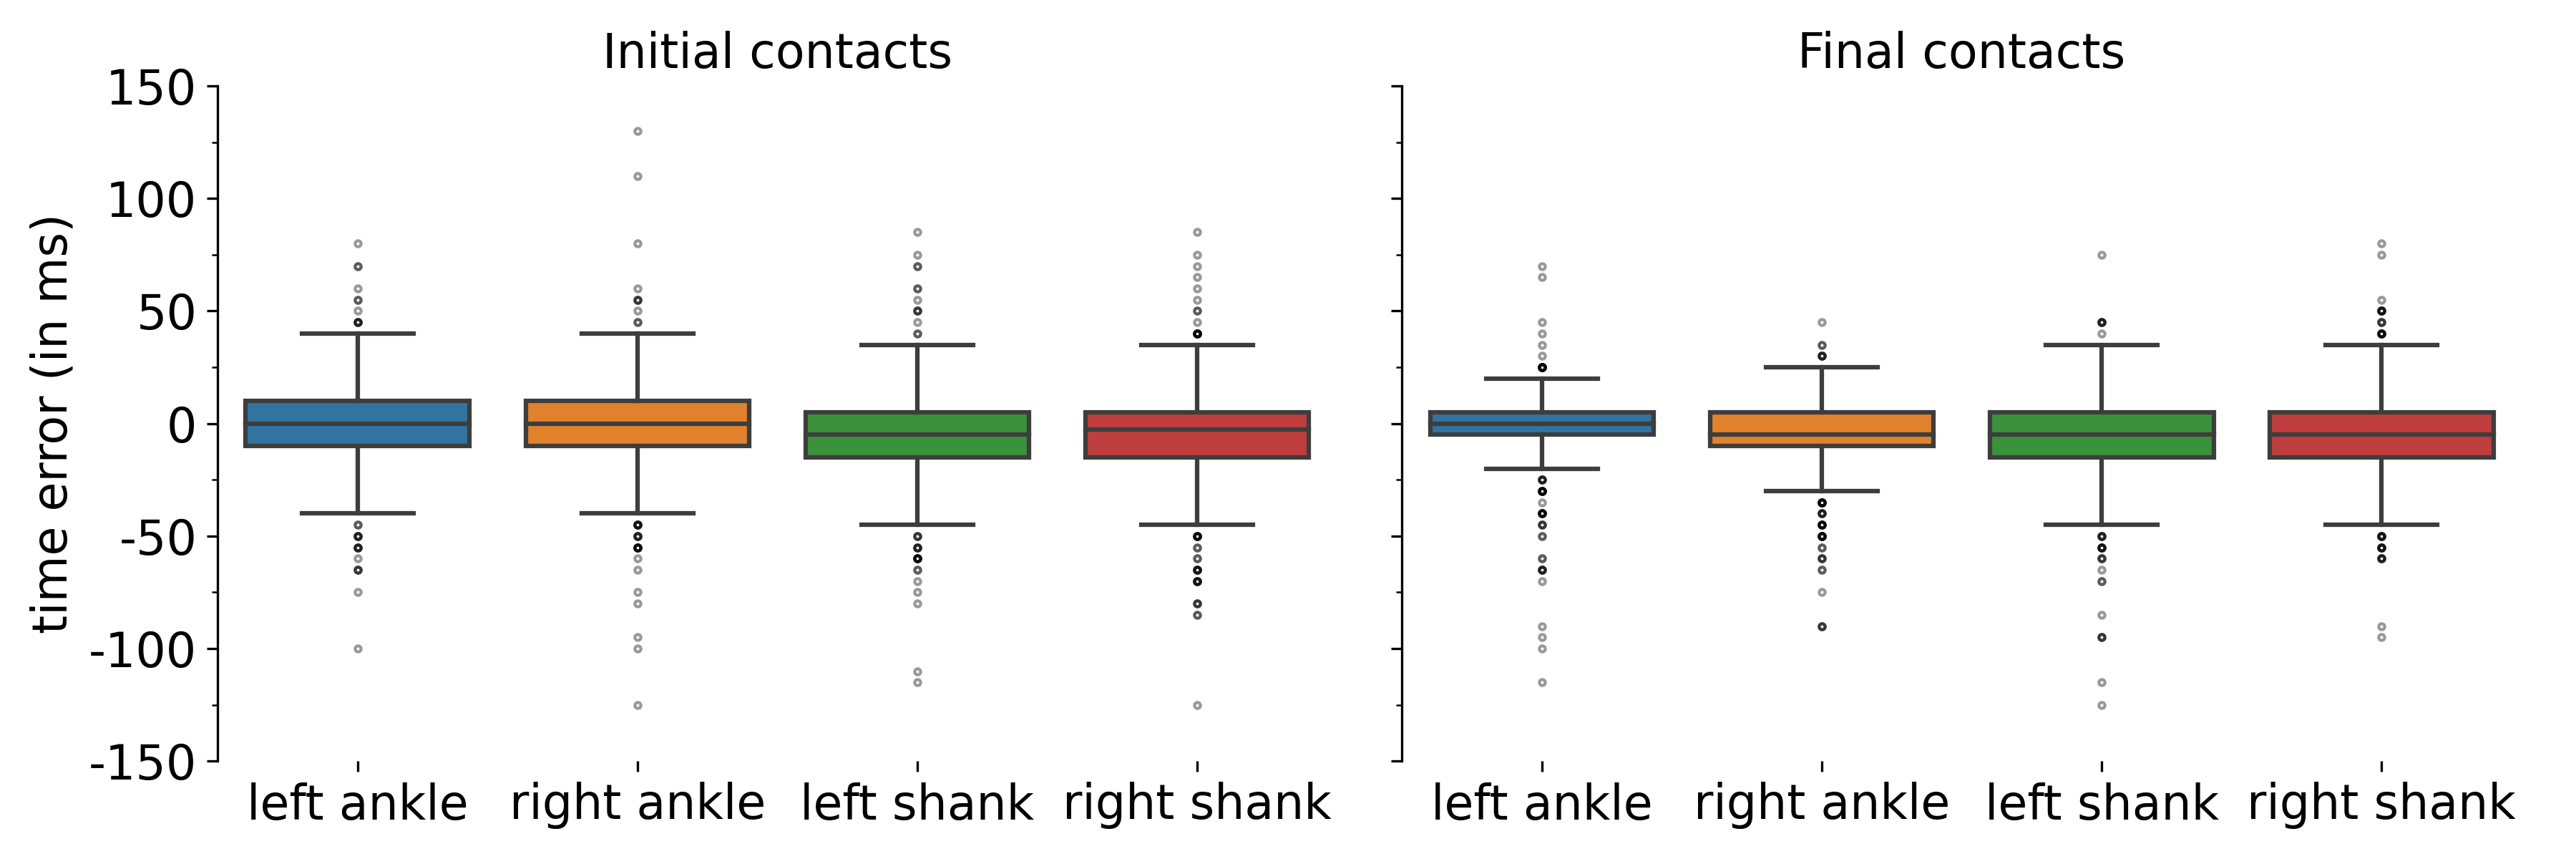
\includegraphics[width=13.5 cm]{fig/box_plots_tracked_points_with_outliers}
	\caption{Time errors for initial (left) and final (right) contacts detection, for each of the different tracked points.\label{fig:time_error_box_plots}}
\end{figure}

Time agreement between the annotated and detected events was quantified for the TPs for each of the sensor locations (Figure~\ref{fig:time_error_box_plots}). The median time error for each of the sensor locations, and for both ICs and FCs was close to zero (Table~\ref{tab:time_errors}), and the largest median time error was -0.005 s, corresponding to one sample period (at a sampling frequency of 200 Hz). The IQR was at most 0.020 s, corresponding to 4 sample periods.
\begin{table}[H] 
	\caption{Time errors for the correctly detected gait events. Note that 0.005 s corresponds to 1 sample period, given the sampling frequency of 200 Hz. \label{tab:time_errors}}
	\newcolumntype{C}{>{\centering\arraybackslash}X}
	\begin{tabularx}{\textwidth}{r|CC|CC}
		\toprule
		 & \multicolumn{2}{c}{\textbf{Initial contacts}} & \multicolumn{2}{c}{\textbf{Final contacts}}\\
		\textbf{Tracked point} & \textbf{median} & \textbf{IQR} & \textbf{median} & \textbf{IQR}\\
		 & s & s & s & s \\
		\midrule
		left ankle & 0.000 & 0.020 & 0.000 & 0.010\\
		right ankle & 0.000 & 0.020 & -0.005 & 0.015\\
		left shank & -0.005 & 0.020 & -0.005 & 0.020\\
		right shank & -0.003 & 0.020 & -0.005 & 0.020\\
		\bottomrule
	\end{tabularx}
	\noindent{\footnotesize{IQR: inter-quartile range.}}
\end{table}

\subsection{Stride-specific Gait Parameters}
For those trials for which all gait events were correctly detected (and no false positives were detected), stride time, stance time and swing time were calculated. The mean difference and the limits of agreement between the marker-based annotations and the model-based detections were calculated.

For all stride-specific gait parameters, and for all sensor locations, the mean difference was close to zero, i.e., the maximum mean difference was 0.003 s, namely for the calcualted swing time of the right ankle (Table~\ref{tab:stride_parameters}). Furthermore, for all gait parameters and for all sensor locations the limits of agreement, based on a 95\% confidence interval were distributed around a zero-mean difference with the overall limits of agreement at -0.049 s and 0.051 s (Figure~\ref{fig:gait_parameters_bland_altman_plots}).
\begin{table}[H] 
	\caption{Time agreement between the stride-specific parameters. \label{tab:stride_parameters}}
	\newcolumntype{C}{>{\centering\arraybackslash}X}
	\begin{tabularx}{\textwidth}{rrCC}
		\toprule
		\textbf{Tracked point} & \textbf{Parameters} & \textbf{Mean difference} & \textbf{Limits of Agreement}\\
		 & & s & (s, s)\\
		\midrule
		left ankle & stride time & 0.001 & (-0.035, 0.036)\\
		 & stance time & 0.002 & (-0.039, 0.042)\\
		 & swing time & -0.001 & (-0.045, 0.043)\\
		\midrule
		right ankle & stride time & 0.000 & (-0.039, 0.040)\\
		 & stance time & -0.002 & (-0.048, 0.044)\\
		 & swing time & 0.003 & (-0.046, 0.051)\\
		\midrule
		left shank & stride time & 0.001 & (-0.039, 0.041)\\
		& stance time & 0.002 & (-0.043, 0.046)\\
		& swing time & -0.001 & (-0.049, 0.047)\\
		\midrule
		right shank & stride time & -0.000 & (-0.031, 0.031)\\
		& stance time & 0.002 & (-0.046, 0.049)\\
		& swing time & -0.002 & (-0.049, 0.046)\\
		\bottomrule
	\end{tabularx}
	\noindent{}
\end{table}

\begin{figure}[H]
	\begin{adjustwidth}{-\extralength}{0cm}
		\centering
		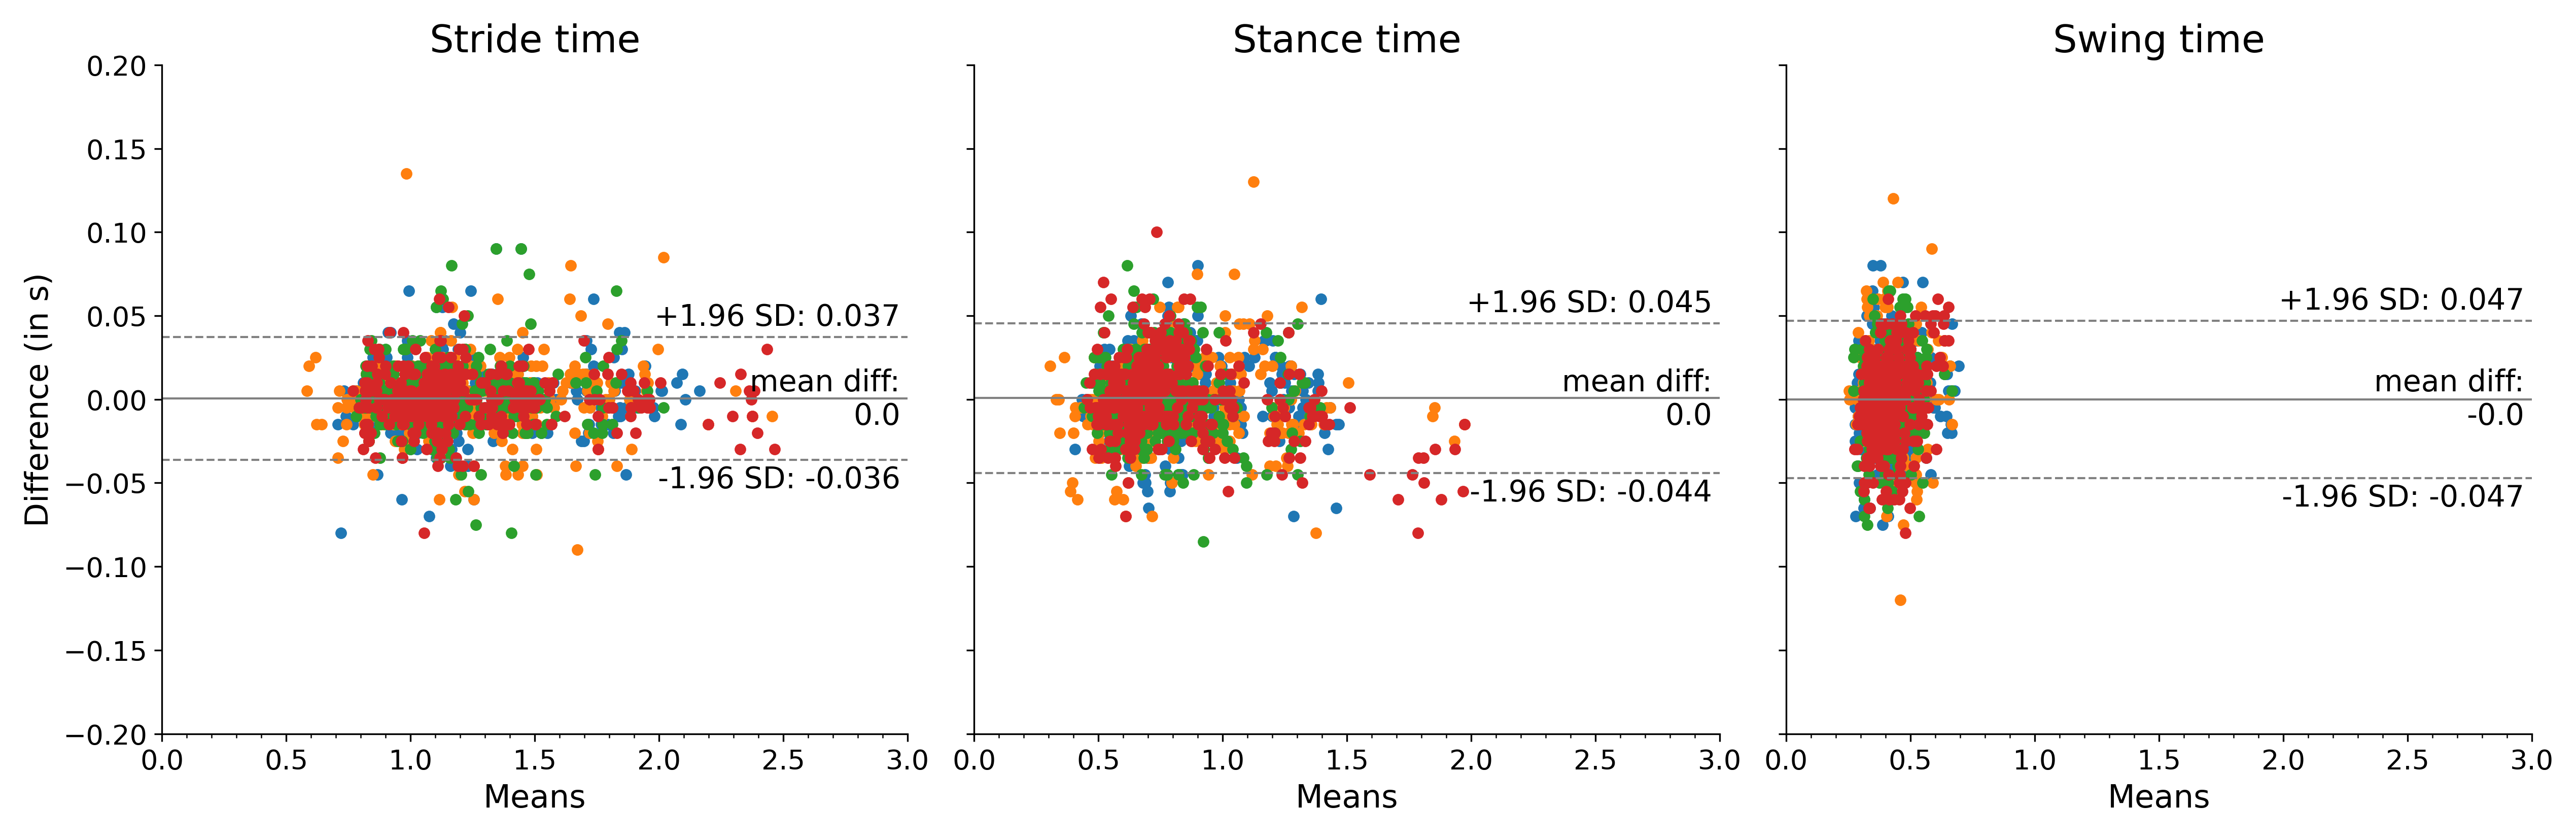
\includegraphics[width=18.5cm]{fig/bland_altman_plots_stride_params}
	\end{adjustwidth}
	\caption{The agreement of extracted gait parameters between the sensor-based and marker-based methods.\label{fig:gait_parameters_bland_altman_plots}}
\end{figure}  


%%%%%%%%%%%%%%%%%%%%%%%%%%%%%%%%%%%%%%%%%%
\section{Discussion}
The current study aimed to validate a deep learning approach for detecting gait events from a single IMU worn on the lower leg. Data from left and right ankle- and shank-worn IMUs were used for training a neural network to detect gait events from walking trials performed by healthy YA, healthy OA, participants diagnosed with PD, MS, or cLBP, participants who had a recent symptomatic stroke, and participants diagnosed with other neurological diseases. Participants walked a 5 meter distance at three different self-selected walking speeds. The gait event timings that were predicted by the neural network were compared to a common reference method, i.e., OMC system, and clinically relevant stride-specific gait parameters were extracted. 

A first measure for the model performance was given by the recall (how many annotated events were detected) and precision (how many detected events were annotated). For both ICs and FCs, a high recall ($\ge 95\%$) and high precision ($\ge 98\%$) were observed, meaning that most events can be detected and most detected events were actually true events. There was little difference in recall and precision between sensor locations (Table~\ref{tab:overall_detection_performance}) confirming that the deep learning approach is relatively invariant to exact sensor localization. 

Next, the time error, that is the difference between the annotated event and the detected event, was of interest. For both ICs and FCs, and for all sensor locations, the observed time error was small, and the middle $50\%$ of the time errors were within a range of $\left[-0.015,0.010\right]$ s (Table~\ref{tab:time_errors}, Figure~\ref{fig:time_error_box_plots}). These data showed that the deep learning-based approach is precise in detecting initial and final contacts. Time errors were slightly smaller than our previously reported results \cite{Romijnders2021} that used a heuristics-based approach \cite{Salarian2004}. The heuristics-based approach determined ICs and FCs as local minima in the medio-lateral angular velocity \cite{Salarian2004} and it could be that these minima do not exactly coincide with the referent event timing as determined from the OMC systems. The median and IQR of the time errors were in the same range as previously found by \cite{Gadaleta2019}. The time errors were lower than previously reported time errors from a continious wavelet-based approach \cite{Ji2019}.

From the correctly detected gait events, stride-specific gait parameters were derived. These are probably of greatest clinical relevance, as changes in stride-specific gait parameters have been linked directly with disease onset and progression \cite{DelDin2019,Koenig2017,Bertoli2018,SchroederVon1995,Mohan2021,Griskevicius2016,Flachenecker2019}. Therefore, stride time, stance time, and swing time were calculated, and the differences between the deep learning-based approach and the marker-based reference method were quantified (Table~\ref{tab:stride_parameters}, Figure~\ref{fig:gait_parameters_bland_altman_plots}). The limits of agreement for a $95\%$ confidence interval were calculated, and for all metrics the zero-mean difference was enclosed in the limit of agreement. These data provided evidence that the deep learning-based model was able to derive stride-specific gait parameters. The differences between the deep learning model-based stride parameters and the marker-based stride parameters were in a similar range as a recent study that compared IMU-derived stride parameters against stride parameters obtained with a pressure sensing walkway \cite{Niswander2021,Gadaleta2019}, and were also in the same range as a study that compared IMU-derived stride parameters with stride parameters obtained with an OMC systems \cite{Carcreff2018}.

The main limitations of the current study were that only walking trials involving straight-line walking were considered, and the walking distance was relatively short. Therefore, it may be that the observed gait patterns from these walking trials are not fully representative of gait patterns observed in daily-life \cite{Hillel2019,Warmerdam2020,Atrsaei2021}. However, as the deep learning-based approach does not rely on fixed thresholds or assumptions to which sensor axis is used, it is theoretically transferable and scalable to other conditions if input data and corresponding labels can be provided. 

%%%%%%%%%%%%%%%%%%%%%%%%%%%%%%%%%%%%%%%%%%
\section{Conclusions}
In this study we have validated a deep learning-based approach to detect gait events and subsequently extract clinically relevant stride-specific gait parameters from a single IMU worn either laterally above the ankle joint or proximal below the knee joint. Performance analysis showed an excellent detection rate, and low time errors in both event detection and stride parameter calculation for different walking speeds and across both healthy and neurological cohorts. Our next step is to validate these methods with real-life walking sequences.

%%%%%%%%%%%%%%%%%%%%%%%%%%%%%%%%%%%%%%%%%%
\vspace{6pt} 

%%%%%%%%%%%%%%%%%%%%%%%%%%%%%%%%%%%%%%%%%%
%% optional
%\supplementary{The following supporting information can be downloaded at:  \linksupplementary{s1}, Figure S1: title; Table S1: title; Video S1: title.}

% Only for the journal Methods and Protocols:
% If you wish to submit a video article, please do so with any other supplementary material.
% \supplementary{The following supporting information can be downloaded at: \linksupplementary{s1}, Figure S1: title; Table S1: title; Video S1: title. A supporting video article is available at doi: link.}

%%%%%%%%%%%%%%%%%%%%%%%%%%%%%%%%%%%%%%%%%%
\authorcontributions{Conceptualization, R.R., G.S., and W.M.; methodology, R.R., G.S.; software, R.R.; validation, R.R.,; formal analysis, R.R.; investigation, R.R., G.S., W.M.; resources, C.H, W.M..; data curation, E.W., R.R.,; writing---original draft preparation, R.R.; writing---review and editing, E.W., C.H., G.S., W.M.; visualization, R.R.; supervision, G.S., W.M.; project administration, R.R., E.W., C.H., G.S., W.M.; funding acquisition, W.M. All authors have read and agreed to the published version of the manuscript.}

\funding{This research received funding from the DFG Open Access fund.}

\institutionalreview{The study was conducted in accordance with the Declaration of Helsinki, and approved by the Ethics Committee of the medical faculty of the Christian-Albrechts-Universit\"{a}t zu Kiel (D438/18, approved on 8 May 2018).}

\informedconsent{Informed consent was obtained from all subjects involved in the study.}

\dataavailability{Data from the first 10 participant are available online at \url{https://github.com/neurogeriatricskiel/Validation-dataset}. Additionally, we are preparing the open-source release of all data from the healthy younger and older adults. Data from patient groups can be shared upon reasonable request.} 

\acknowledgments{The authors sincerely thank all people that were involved in the data collection, from study participants to students who aided and assisted during measurements and subsequent marker labeling. The authors thank Julius Welzel for his input regarding the organization of the data in a BIDS-like format. The authors thank Johannes Hoffmann for his tips regarding the \LaTeX typesetting.}

\conflictsofinterest{The authors declare no conflict of interest.} 

%% Optional
% \sampleavailability{Samples of the compounds ... are available from the authors.}

%%%%%%%%%%%%%%%%%%%%%%%%%%%%%%%%%%%%%%%%%%
%% Only for journal Encyclopedia
%\entrylink{The Link to this entry published on the encyclopedia platform.}

%%%%%%%%%%%%%%%%%%%%%%%%%%%%%%%%%%%%%%%%%%
%% Optional
\abbreviations{Abbreviations}{
The following abbreviations are used in this manuscript:\\

\noindent 
\begin{tabular}{@{}ll}
	cLBP & chronic low back pain\\
	CNN & convolutional neural network\\
	IMU & inertial measurement unit\\
	MS & multiple sclerosis\\
	OA & older adults\\
	PD & Parkinson's Disease\\
	TCN & temporal convolutional network\\
	YA & younger adults
\end{tabular}}

%%%%%%%%%%%%%%%%%%%%%%%%%%%%%%%%%%%%%%%%%%
%%% Optional
%\appendixtitles{no} % Leave argument "no" if all appendix headings stay EMPTY (then no dot is printed after "Appendix A"). If the appendix sections contain a heading then change the argument to "yes".
%\appendixstart
%\appendix
%\section[\appendixname~\thesection]{}
%\subsection[\appendixname~\thesubsection]{}
%The appendix is an optional section that can contain details and data supplemental to the main text---for example, explanations of experimental details that would disrupt the flow of the main text but nonetheless remain crucial to understanding and reproducing the research shown; figures of replicates for experiments of which representative data are shown in the main text can be added here if brief, or as Supplementary Data. Mathematical proofs of results not central to the paper can be added as an appendix.
%
%\begin{table}[H] 
%\caption{This is a table caption.\label{tab5}}
%\newcolumntype{C}{>{\centering\arraybackslash}X}
%\begin{tabularx}{\textwidth}{CCC}
%\toprule
%\textbf{Title 1}	& \textbf{Title 2}	& \textbf{Title 3}\\
%\midrule
%Entry 1		& Data			& Data\\
%Entry 2		& Data			& Data\\
%\bottomrule
%\end{tabularx}
%\end{table}
%
%\section[\appendixname~\thesection]{}
%All appendix sections must be cited in the main text. In the appendices, Figures, Tables, etc. should be labeled, starting with ``A''---e.g., Figure A1, Figure A2, etc.

%%%%%%%%%%%%%%%%%%%%%%%%%%%%%%%%%%%%%%%%%%
\begin{adjustwidth}{-\extralength}{0cm}
%\printendnotes[custom] % Un-comment to print a list of endnotes

\reftitle{References}

% Please provide either the correct journal abbreviation (e.g. according to the “List of Title Word Abbreviations” http://www.issn.org/services/online-services/access-to-the-ltwa/) or the full name of the journal.
% Citations and References in Supplementary files are permitted provided that they also appear in the reference list here. 

%=====================================
% References, variant A: external bibliography
%=====================================
%\bibliography{your_external_BibTeX_file}

%=====================================
% References, variant B: internal bibliography
%=====================================
\begin{thebibliography}{999}
	\bibitem[Snijders(2007)]{Snijders2007}
	Snijders,~A.H.; {van de Warrenburg},~B.P.; Giladi,~N.; Bloem,~B.R. Neurological gait disorders in elderly people: clinical approach and classification. {\em Lancet Neurol.} {\bf 2007}, {\em 6}(1), 63--74.
	\bibitem[Hodgins(2008)]{Hodgins2008}
	Hodgins,~D. The importance of measuring human gait. {\em Med. Device Technol.} {\bf 2008}, {\em 19}(5):42, 44-7.
	\bibitem[DelDin(2019)]{DelDin2019}
	{Del Din},~S.; Elshehabi,~M.; Galna,~B.; Hobert,~M.A.; Warmerdam,~E.; Suenkel,~U.; Brockmann,~K.; Metzger,~F.; Hansen,~C.; Berg,~D.; Rochester,~L.; Maetzler,~W. Gait analysis with wearables predicts conversion to Parkinson disease. {\em Ann. Neurol.} {\bf 2019}, {\em 86}(3), 357--367.
	\bibitem[Koenig(2017]{Koenig2017}
	K\"{o}nig,~A.; Klaming,~L.; Pijl,~M.; Demeurraux,~A.; Davis,~R.; Robert,~P. Objective measurement of gait parameters in healthy and cognitively impaired elderly using the dual-task paradigm. {\em Aging. Clin. Exp. Res.} {\bf 2017}, {\em 29}(6), 1181--1189.
	\bibitem[Bertoli(2018)]{Bertoli2018}
	Bertoli,~M.; Cereatti,~A.; Trojaniello,~D.; Avanzino,~L.; Pelosin,~E.; Del Din,~S.; Rochester,~L.; Ginis,~P.; Bekkers,~E.M.J.; Mirelman,~A.; Hausdorff,~J.M.; {Della Croce},~U. Estimation of spatio-temporal parameters of gait from magneto-inertial measurement units: multicenter validation among Parkinson, mildly cognitively impaired and healthy older adults. {\em Biomed. Eng. Online} {\bf 2018}, {\em 17}(58).
	\bibitem[SchroederVon(1995)]{SchroederVon1995}
	von Schroeder,~H.P.; Coutts,~R.D.; Lyden,~P.D.; Billings,~E.,~Jr; Nickel,~V. L. Gait parameters following stroke: a practical assessment. {\em J. Rehabil. Res. Dev.} {\bf 1995}, {\em 32}(1), 25--31.
	\bibitem[Mohan(2021)]{Mohan2021}
	Mohan,~D.M.; Khandoker,~A.H.; Wasti,~S.A.; Ismail~Ibrahim~Ismail~Alali,~S.; Jelinek,~H.F.; Khalaf,~K. Assessment methods of post-stroke gait: A scoping review of technology-driven approaches to gait characterization and analysis. {\em Front. Neurol.} {\bf 2021}, {\em 12}.
	\bibitem[Griskevicius(2016)]{Griskevicius2016}
	Gri\v{s}kevi\v{c}ius,~J.; Apanskien\.{e},~V.; \v{Z}i\v{z}ien\.{e},~J.; Daunoravi\v{c}ien\.{e},~K.; Ov\v{c}inikova,~A.; Kizlaitien\.{e},~R.; Sereik\.{e},~I.; Kaubrys,~G.; Pauk,~J.; Id\'{z}kowski,~A. Estimation of temporal gait parameters of multiple sclerosis patients in clinical setting using inertial sensors. In Proceedings of the 11th Int Conf BIOMDLORE 2016, Druskininkai, Lithuania, 20--22 Oct 2016; 80--82.
	\bibitem[Flachenecker(2019)]{Flachenecker2019}
	Flachenecker,~F.; Ga{\ss}ner,~H.; Hannik,~J.; Lee,~D.H.; Flachenecker,~P.; Winkler,~J.; Eskofier,~B.; Linker,~R.A.; Klucken,~J. Objective sensor-based gait measures reflect motor impairment in multiple sclerosis patients: Reliability and clinical validation of a wearable sensor device. {\em Mult. Scler. Relat. Dis.} {\bf 2019}, {\em 39}, 101903.
	\bibitem[Hannink(2016)]{Hannink2016}
	Hannink,~J.; Kautz,~T.; Pasluosta,~C.F.; Ga{\ss}mann,~K.-G.; Klucken,~J.; Eskofier,~B.M. Sensor-Based Gait Parameter Extraction With Deep Convolutional Neural Networks. {\em IEEE J. Biomed. Health} {\bf 2017}, {\em 21}(1), 85--93.
	\bibitem[Perry(2010)]{Perry2010}
	Perry,~J; Burnfield,~J.M. \textit{Gait analysis: normal and pathological gait}, 2nd ed.; SLACK Inc.: Thorofare, NJ, USA, 2010.
	\bibitem[Whittle(2012)]{Whittle2012}
	Richards,~J.; Levine,~D.; Whittle,~M. \textit{Whittle's Gait Analysis}, 5th ed.; Churchill Livingstone: London, UK, 2012.
	\bibitem[Rueterbories(2010)]{Rueterbories2010}
	Rueterbories,~J.; Spaich,~E.G.; Larsen,~B.; Andersen,~O.K. Methods for gait event detection and analysis in ambulatory systems. {\em Med. Eng. Phys.} {\bf 2010}, {\em 32}(6), 545--552.
	\bibitem[Bruening(2014)]{Bruening2014}
	Bruening,~D.A.; Ridge,~S.T. Automated event detection algorithms in pathological gait. {\em Gait Posture} {\bf 2014}, {\em 39}(1), 472--477.
	\bibitem[Chiari(2005)]{Chiari2005}
	Chiari,~L.; Della~Croce,~U.; Leardini,~A.; Cappozzo,~A. Human movement analysis using stereophotogrammetry: Part 2: Instrumental errors {\em Gait Posture} {\bf 2005}, {\em 21}(2), 197--211.
	\bibitem[Topley(2020)]{Topley2020}
	Topley,~M.; Richards,~J.G. A A comparison of currently available optoelectronic motion capture systems. {\em J. Biomech.} {\bf 2020}, {\em 106}:109820.	
	\bibitem[Iosa(2016)]{Iosa2016}
	Iosa,~M.; Picerno,~P.; Paolucci,~S.; Morone,~G. Wearable inertial sensors for human movement analysis. {\em Expert Rev. Med. Devic.} {\bf 2016}, {\em 13}(7), 641--659.
	\bibitem[Jarchi(2018)]{Jarchi2018}
	Jarchi,~D.; Pope,~J.; Lee,~T.K.M.; Tamjidi,~L.; Mirzaei,~A.; Sanei,~S. A Review on Accelerometry-Based Gait Analysis and Emerging Clinical Applications. {\em IEEE Rev. Biomed. Eng.} {\bf 2018}, {\em 11}, 177--194.
	\bibitem[Hillel(2019)]{Hillel2019}
	Hillel,~I; Gazit,~E.; Nieuwboer,~A.; Avanzino,~L.; Rochester,~L.; Cereatti,~A.; Della~Croce,~U.; Rikkert,~M.O.; Bloem,~B.R.; Pelosin,~E.; Del~Din,~S.; Ginis,~P.; Giladi,~N.;  Mirelman,~A.; Hausdorff,~J.M. Is every-day walking in older adults more analogous to dual-task walking or to usual walking? Elucidating the gaps between gait performance in the lab and during 24/7 monitoring. {\em Eur. Rev. Aging Phys. A.} {\bf 2019}, {\em 16}(6).
	\bibitem[Warmerdam(2020)]{Warmerdam2020}
	Warmerdam,~E.; Hausdorff,~J.M.; Atrsaei,~A.; Zhou,~Y.; Mirelman,~A.; Aminian,~K.; Espay,~A.J.; Hansen,~C.; Evers,~L.J.W.; Keller,~A.; Lamoth,~C.; Pilotto,~A.; Rochester,~L.; Schmidt,~G.; Bloem,~B.R.; Maetzler,~W. Long-term unsupervised mobility assessment in movement disorders. {\em Lancet Neurol.} {\bf 2020}, {\em 19}(5), 462--470.
	\bibitem[Atrsaei(2021)]{Atrsaei2021}
	Atrsaei,~A.; Corr\'{a},~M.F.; Dadashi,~F.; Vila-Ch\~{a},~N.; Maia,~L.; Mariani,~B.; Maetzler,~W.; Aminian,~K. Gait speed in clinical and daily living assessments in Parkinson’s disease patients: performance versus capacity. {\em npj Parkinsons Dis.} {\bf 2021}, {\em 7}(1):24.
	\bibitem[DelDin(2016)]{DelDin2016}
	Del~Din,~S.; Godfrey,~A.; Mazz\`{a},~C.; Lord,~S.; Rochester,~L. Free-living monitoring of Parkinson's disease: Lessons from the field. {\em Movement Disord.} {\bf 2016}, {\em 31}(9), 1293--1313.
	\bibitem[Shah(2020)]{Shah2020}
	Shah,~V.V.; McNames,~J.; Mancini,~M.; Carlson-Kuhta,~P.; Nutt,~J.G.; El-Gohary,~M.; Lapidus,~J.A.; Horak,~F.B.; Curtze,~C. Digital Biomarkers of Mobility in Parkinson's Disease During Daily Living. {\em J. Parkinson Dis.} {\bf 2020}, {\em 10}(3), 1099--1111.
	\bibitem[Fasano(2020)]{Fasano2020}
	Fasano,~A.; Mancini,~M. Wearable-based mobility monitoring: the long road ahead. {\em Lancet Neurol.} {\bf 2020}, {\em 19}(5), 378--379.
	\bibitem[Corra(2021)]{Corra2021}
	Corr\'{a},~M.F.; Atrsaei,~A.; Sardoreira,~A.; Hansen,~C.; Aminian,~K.; Correia,~M.; Vila-Ch\~{a},~N.; Maetzler,~W.; Maia,~L. Comparison of Laboratory and Daily-Life Gait Speed Assessment during ON and OFF States in Parkinson’s Disease. {\em Sensors} {\bf 2021}, {\em 21}(12):3974.
	\bibitem[BenMansour(2015)]{BenMansour2015}
	Ben~Mansour,~K.; Rezzoug,~N.; Gorce,~P. Analysis of several methods and inertial sensors locations to assess gait parameters in able-bodied subjects. {\em Gait Posture} {\bf 2015}, {\em 42}, 409--414.
	\bibitem[Storm(2016)]{Storm2016}
	Storm,~F.A.; Buckley,~C.J.; Mazz\`{a},~C. Gait event detection in laboratory and real life settings: Accuracy of ankle and waist sensor based methods. {\em Gait Posture} {\bf 2016}, {\em 50}, 42--46.
	\bibitem[Panebianco(2018)]{Panebianco2018}
	Panebianco,~G.P.; Bisi,~M.C.; Stagni,~R.; Fantozzi,~S. Analysis of the performance of 17 algorithms from a systematic review: Influence of sensor position, analysed variable and computational approach in gait timing estimation from IMU measurements. {\em Gait Posture} {\bf 2018}, {\em 66}, 76--82.
	\bibitem[Niswander(2021)]{Niswander2021}
	Niswander,~W.; Kontson,~K. Evaluating the Impact of IMU Sensor Location and Walking Task on Accuracy of Gait Event Detection Algorithms. {\em Sensors} {\bf 2021}, {\em 21}(12):3989.
	\bibitem[Salarian(2004)]{Salarian2004}
	Salarian,~A.; Russmann,~H.; Vingerhoets,~F.J.; Dehollain,~C.; Blanc,~Y.; Burkhard,~P.R.; Aminian,~K. Gait assessment in Parkinson's
	disease: Toward an ambulatory system for long-term monitoring. {\em IEEE Trans. Biomed. Eng.} {\bf 2004}, {\em 51}(8), 1434--1443. 
	\bibitem[Catalfamo(2010)]{Catalfamo2010}
	Catalfamo,~P.; Ghoussayni,~S.; Ewins,~D. Gait Event Detection on Level Ground and Incline Walking Using a Rate Gyroscope. {\em Sensors} {\bf 2010}, {\em 10}(6), 5683--5702. 
	\bibitem[Sabatini(2005)]{Sabatini2005}
	Sabatini,~A.; Martelloni,~C.; Scapellato,~S.; Cavallo,~F. Assessment of Walking Features from Foot Inertial Sensing. {\em IEEE Trans. Biomed. Eng.} {\bf 2005}, {\em 52}(3), 486--494.
	\bibitem[Maqbool(2016)]{Maqbool2016}
	Maqbool,~H.F.; Husman,~M.A.B.; Awad,~M.; Abouhossein,~A.; Mehryar,~P.; Iqbal,~N.; Dehghani-Sanij,~A.A. Real-time gait event detection for lower limb amputees using a single wearable sensor. In Proceedings of the 2016 38th Ann. Int. Conf. of the IEEE Eng. in Med. Biol. Soc. (EMBC), Orlando, FL, USA, 16--20 Aug. 2016, IEEE: Piscataway, NJ, USA, 2016. 
	\bibitem[Romijnders(2021)]{Romijnders2021}
	Romijnders,~R.; Warmerdam,~E.; Hansen,~C.; Welzel,~J.; Schmidt,~G.; Maetzler,~W. Validation of IMU-based gait event detection during curved walking and turning in older adults and Parkinson's Disease patients. {\em J. Neuroeng. Rehabil.} {\bf 2021}, {\em 18}:28.
	\bibitem[Jasiewicz(2006)]{Jasiewicz2006}
	Jasiewicz,~J.M.; Allum,~J.H.; Middleton,~J.W.; Barriskill,~A.; Condie,~P.; Purcell,~B.; Li,~R.C.T. Gait event detection using linear accelerometers or angular velocity transducers in able-bodied and spinal-cord injured individuals. {\em Gait Posture} {\bf 2006}, {\em 24}(4), 502--509.
	\bibitem[Trojaniello(2014)]{Trojaniello2014}
	Trojaniello,~D.; Cereatti,~A.; Pelosin,~E.; Avanzino,~L.; Mirelman,~A.; Hausdorff,~J.M.; Della~Croce,~U. Estimation of step-by-step spatio-temporal parameters of normal and impaired gait using shank-mounted magneto-inertial sensors: Application to elderly, hemiparetic, parkinsonian and choreic gait. {\em J. Neuroeng. Rehabil.} {\bf 2014}, {\em 11}:152.
	\bibitem[Ferraris(1995)]{Ferraris1995}
	Ferraris,~F.; Grimaldi,~U.; Parvis,~M. Procedure for effortless in-field calibration of three-axis rate gyros and accelerometers. {\em Sensor. Mater.} {\bf 1995}, {\em 7}(5), 311--330.
	\bibitem[Greene(2010)]{Greene2010}
	Greene,~B.R.; McGrath,~D.; O'Neill,~R.; O'Donovan,~K.J.; Burns,~A.; Caulfield,~B. An adaptive gyroscope-based algorithm for temporal gait analysis. {\em Med. Biol. Eng. Comput.} {\bf 2010}, {\em 48}(12), 1251--1260.
	\bibitem[Leineweber(2019)]{Leineweber2019}
	Leineweber,~M.J.; Gomez~Orozco,~M.~D.; Andrysek,~J. Evaluating the feasibility of two post-hoc correction techniques for mitigating posture-induced measurement errors associated with wearable motion capture. {\em Med. Eng. Phys.} {\bf 2019}. {\em 71}:38–44.
	\bibitem[Pacher(2020)]{Pacher2020}
	Pacher,~L.; Chatellier,~C.; Vauzelle,~R.; Fradet,~L. Sensor-to-Segment Calibration Methodologies for Lower-Body Kinematic Analysis with Inertial Sensors: A Systematic Review. {\em Sensors} {\bf 2020}, {\em 20}(11):3322.	
	\bibitem[LeCun(2015)]{LeCun2015}
	LeCun,~Y.; Bengio,~Y.; Hinton,~G. Deep learning. {\em Nature} {\bf 2015}, {\em 521}, 436-444.
	\bibitem[TerHaarRomeny(2019)]{TerHaarRomeny2019}
	Ter Haar Romeny,~B.M. A Deeper Understanding of Deep Learning. In {\em Artificial Intelligence in Medical Imaging: Opportunities, Applications and Risks}; Ranschaert,~E.R., Morozov,~S., Algra,~P.R., Eds.; Springer Int. Publish.: Cham, Switzerland, 2019; pp. 25--38.	
	\bibitem[Kidzinski(2019)]{Kidzinski2019}
	Kidzi\'{n}ski,~{\L}.; Delp,~S.; Schwartz,~M. Automatic real-time gait event detection in children using deep neural networks. {\em PLoS ONE} {\bf 2019}, {\em 14}(1):e0211466.
	\bibitem[Lempereur(2020)]{Lempereur2020}
	Lempereur,~M.; Rousseau,~F.; R\'{e}my-N\'{e}ris,~O.; Pons,~C.; Houx,~L.; Quellec,~G.; Brochard,~S. A new deep learning-based method for the detection of gait events in children with gait disorders: Proof-of-concept and concurrent validity. {\em J. Biomech.} {\bf 2020}, {\em 98}, 109490.
	\bibitem[Filtjens(2020)]{Filtjens2020}
	Filtjens,~B.; Nieuwboer,~A.; D'cruz,~N.; Spildooren,~J.; Slaets,~P.; Vanrumste,~B. A data-driven approach for detecting gait events during turning in people with Parkinson's disease and freezing of gait. {\em Gait Posture} {\bf 2020}, {\em 80}, 130--136.
	\bibitem[Gadaleta(2019)]{Gadaleta2019}
	Gadaleta,~M.; Cisotto,~G.; Rossi,~M.; Ur~Rehman,~R.Z.; Rochester,~L.; Del~Din,~S. Deep Learning Techniques for Improving Digital Gait Segmentation. In Proceedings of the 2019 41st Ann. Int. Conf. of the IEEE Eng. in Med. Biol. Soc. (EMBC), Berlin, Germany, 23--27 Jul. 2019, IEEE: Piscataway, NJ, USA, 2019.
	
	% Materials and Methods
	\bibitem[Warmerdam(2021)]{Warmerdam2021}
	Warmerdam,~E.; Romijnders,~R.; Geritz,~J.; Elshehabi,~M.; Maetzler,~C.; Otto,~J.C.; Reimer,~M.; Stuerner,~K.; Baron,~R.; Paschen,~S.; Beyer,~T.; Dopcke,~D.; Eiken,~T.; Ortmann,~H.; Peters,~F.; von~der~Recke,~F.; Riesen,~M.; Rohwedder,~G.; Schaade,~A.; Schumacher,~M.; Sondermann,~A; Maetzler,~W.; Hansen,~C. Proposed Mobility Assessments with Simultaneous Full-Body Inertial Measurement Units and Optical Motion Capture in Healthy Adults and Neurological Patients for Future Validation Studies: Study Protocol. {\em Sensors} {\bf 2021}, {\em 21}(17):5833.
	\bibitem[Gibb(1988)]{Gibb1988}
	Gibb,~W.R.; Lees,~A.J. The relevance of the Lewy body to the pathogenesis of idiopathic Parkinson's disease. {\em J. Neurol. Neurosur. Ps.} {\bf 1988}, {\em 51}(6), 745--752.
	\bibitem[Thompson(2018)]{Thompson2018}
	Thompson,~A.J.; Banwell,~B.L.; Barkhof,~F.; Carroll,~W.M.; Coetzee,~T.; Comi,~G.; Correale,~J.; Fazekas,~F.; Filippi,~M.; Freedman,~M.S.; Fujihara,~K.; Galetta,~S.L.; Hartung,~H.P.; Kappos,~L.; Lublin,~F.D.; Marrie,~R.A.; Miller,~A.E.; Miller,~D.H.; Montalban,~X.; Mowry,~E.M.; Soelberg~Sorensen,~P.; Tintor\'{e},~M.; Traboulsee,~A.L.; Trojano,~M.; Uitdehaag,~B.M.J.; Vukusic,~S.; Waubant,~E.; Weinshenker,~B.G.; Reingold,~S.C.; Cohen,~J.A. Diagnosis of multiple sclerosis: 2017 revisions of the McDonald criteria. {\em Lancet Neurol.} {\bf 2018}, {\em 17}(2), 162--173.
	\bibitem[Nasreddine(2005)]{Nasreddine2005}
	Nasreddine,~Z.S.; Phillips,~N.A.; B\'{e}dirian,~V.; Charbonneau,~S.; Whitehead,~V.; Collin,~I.; Cummings,~J.L.; Chertkow,~H. The Montreal Cognitive Assessment, MoCA: A Brief Screening Tool For Mild Cognitive Impairment. {\em J. Am. Geriatr. Soc.} {\bf 2005}, {\em 53}(4), 695--699.
	\bibitem[Federolf(2013)]{Federolf2013}
	Federolf,~P.A. A Novel Approach to Solve the “Missing Marker Problem” in Marker-Based Motion Analysis That Exploits the Segment Coordination Patterns in Multi-Limb Motion Data. {\em PLoS ONE} {\bf 2013}, {\em 8}(10), 1--13.
	\bibitem[Gloersen(2016)]{Gloersen2016}
	Gl{\o}ersen,~{\O}; Federolf,~P. Predicting Missing Marker Trajectories in Human Motion Data Using Marker Intercorrelations. {\em PLoS ONE} {\bf 2016}, {\em 11}(3), 1--14.
	\bibitem[Kormylo(1974)]{Kormylo1974}
	Kormylo,~J.; Jain,~V. Two-pass recursive digital filter with zero phase shift. {\em IEEE T. Acoust. Speech} {\bf 1974}, {\em 22}(5), 384--387.
	\bibitem[Racz(2021)]{Racz2021}
	R\'{a}cz,~K.; Rita,~M.K. Marker displacement data filtering in gait analysis: A technical note. {\em Biomed. Signal Proces.} {\bf 2021}, {\em 70}:102974.
	\bibitem[Pijnappels(2001)]{Pijnappels2001}
	Pijnappels,~M.; Bobbert,~M.F.; Van Die\"{e}n,~J.H. Changes in walking pattern caused by the possibility of a tripping reaction. {\em Gait Posture} {\bf 2001}, {\em 14}(1), 11--18.
	\bibitem[OConnor(2007)]{OConnor2007}
	O'Connor,~C.M.; Thorpe,~S.K.; O'Malley,~M.J.; Vaughan,~C.L. Automatic detection of gait events using kinematic data. {\em Gait Posture} {\bf 2007}, {\em 25}(3), 469--474.
	\bibitem[Carcreff(2018)]{Carcreff2018}
	Carcreff,~L.; Gerber,~C.; Paraschiv-Ionescu,~A.; De~Coulon,~G,; Newman,~C.; Armand,~S.; Aminian,~K. What is the best configuration of wearable sensors
	to measure spatiotemporal gait parameters in children with cerebral palsy? {\em Sensors} {\bf 2018}, {\em 18}(2):394.
	\bibitem[YuKoltun(2016)]{YuKoltun2016}
	Yu,~F.; Koltun,~V. Multi-Scale Context Aggregation by Dilated Convolutions. In Proceedings of the 4th Int. Conf. on Learning Representations (ICLR), San Juan, Puerto Rico, 2--4 May 2016, Conference Track Proceedings, 2016.
	\bibitem[Bai(2018)]{Bai2018}
	Bai,~S.; Kolter,~J.Z.; Koltun,~V. An Empirical Evaluation of Generic Convolutional and Recurrent Networks for Sequence Modeling. {\em arXiv:1803.01271} {\bf 2018}.
	\bibitem[Remy(2020)]{Remy2020}
	R\'{e}my,~P. Temporal Convolutional Networks for Keras. {\em GitHub repository} {\bf 2020}, {\em GitHub}, \url{https://github.com/philipperemy/keras-tcn}.
	\bibitem[LeCun(1989)]{LeCun1989}
	LeCun,~Y.; Boser,~B.; Denker,~J.S.; Henderson,~D.; Howard,~R.E.; Hubbard,~W.; Jackel,~L.D. Backpropagation Applied to Handwritten Zip Code Recognition. {\em Neural Comput.} {\bf 1989}, {\em 1}(4), 541--551.
	\bibitem[Ioffe(2015)]{Ioffe2015}
	Ioffe,~S.; Szegedy,~C. Batch Normalization: Accelerating Deep Network Training by
	Reducing Internal Covariate Shift. {\em arXiv:1502.03167} {\bf 2015}.
	\bibitem[Srivastava(2014)]{Srivastava2014}
	Srivastava,~N.; Hinton,~G.; Krizhevsky,~A.; Sutskever,~I.; Salakhutdinov,~R. Dropout: a
	simple way to prevent neural networks from overfitting. {\em J. Mach. Learn. Res.} {\bf 2014} {\em 15}, 1929--1958.
	\bibitem[VanRossum(2009)]{VanRossum2009}
	van~Rossum,~G.; Drake,~F.L. {\em Python 3 Reference Manual}; CreateSpace, Scotts Valley, CA, USA, 2009.
	\bibitem[Chollet(2015)]{Chollet2015}
	Chollet,~F. and others. Keras. {\bf 2015}. \url{https://keras.io}.
	\bibitem[Lea(2017)]{Lea2017}
	Lea,~C.; Flynn,~M.D.; Vidal,~R.; Reiter,~A.; Hager,~G.D. Temporal convolutional networks for action segmentation and detection. In Proceedings of the IEEE Conference on Computer Vision and Pattern Recognition, Honolulu, HI, USA, 22--25 Jul. 2017; p. 156--165.
	\bibitem[VanDenOord(2016)]{VanDenOord2016}
	van~den~Oord,~A.; Dieleman,~S.; Zen,~H.; Simonyan,~K.; Vinyals,~O.; Graves,~A.; Kalchbrenner,~N.; Senior,~A.W.; Kavukcuoglu,~K. WaveNet: A generative model for raw audio. {\em arXiv:1609.03499} {\bf 2016}.
	\bibitem[OMalley(2019)]{OMalley2019}
	O'Malley,~T.; Bursztein,~E.; Long,~J.; Chollet,~F.; Jin,~H.; Invernizzi,~L.; and others; KerasTuner. {\em GitHub repository} {\bf 2019}, {\em GitHub}, \url{https://github.com/keras-team/keras-tuner}.
	\bibitem[Kingma(2014)]{Kingma2014}
	Kingma,~D.P.; Ba,~J. Adam: A Method for Stochastic Optimization {\em arXiv:1412.6980v9} {\bf 2014}.
	\bibitem[Schmidt(2021)]{Schmidt2021}
	Schmidt,~R.M.; Schneider,~F.; Henning,~P. Descending through a crowded valley-benchmarking deep learning optimizers. In Proceedings of the 38th Int. Conf. on Machine Learning (ICML), {\em online}, 18--24 Jul. 2021, pp. 9367--9376.
	\bibitem[Bergstra(2012)]{Bergstra2012}
	Bergstra,~J.; Bengio,~Y. Random Search for Hyper-Parameter Optimization. {\em J. Mach. Learn. Res.} {\bf 2012}, {\em 13}(10), 281--305.
	\bibitem[OpenIntro(2019)]{OpenIntro2019}
	Diez,~D.; \c{C}etinkaya-Rundel,~M.; Barr,~C.D. \textit{OpenIntro Statistics}, 4th ed.; 2019. \url{https://www.openintro.org/book/os/}
	\bibitem[Ji(2019)]{Ji2019}
	Ji,~N.; Zhou,~H.; Guo,~K.; Samuel,~O.W.; Huang,~Z.; Xu,~L.; Li,~G. Appropriate Mother Wavelets for Continuous Gait Event Detection Based on Time-Frequency Analysis for Hemiplegic and Healthy Individuals. {\em Sensors} {\bf 2019}, {\em 19}(16):3462.
	
	\bibitem[Mishra(2019)]{Mishra2019}
	Mishra,~P.; Pandey,~C.M.; Singh,~U.; Gupta,~A.; Sahu,~C.; Keshri,~A. Descriptive Statistics and Normality Tests for Statistical Data. {\em Ann. Card. Anaesth.} {\bf 2019}, {\em 22}(1), 67--72. 	
	\bibitem[Wilcoxon(1945)]{Wilcoxon1945}
	Wilcoxon,~F. Individual Comparisons by Ranking Methods. {\em Biometrics Bull.} {\bf 1945}, {\em 1}, 80--83.
	\bibitem[McDonald(2014)]{McDonald2014}
	McDonald,~J.H. \textit{Handbook of Biological Statistics}, 3rd ed.; Sparky House Publishing: Sparky House Publishing, USA, 2014; pp. 186--189.
\end{thebibliography}

% If authors have biography, please use the format below
%\section*{Short Biography of Authors}
%\bio
%{\raisebox{-0.35cm}{\includegraphics[width=3.5cm,height=5.3cm,clip,keepaspectratio]{Definitions/author1.pdf}}}
%{\textbf{Firstname Lastname} Biography of first author}
%
%\bio
%{\raisebox{-0.35cm}{\includegraphics[width=3.5cm,height=5.3cm,clip,keepaspectratio]{Definitions/author2.jpg}}}
%{\textbf{Firstname Lastname} Biography of second author}

% For the MDPI journals use author-date citation, please follow the formatting guidelines on http://www.mdpi.com/authors/references
% To cite two works by the same author: \citeauthor{ref-journal-1a} (\citeyear{ref-journal-1a}, \citeyear{ref-journal-1b}). This produces: Whittaker (1967, 1975)
% To cite two works by the same author with specific pages: \citeauthor{ref-journal-3a} (\citeyear{ref-journal-3a}, p. 328; \citeyear{ref-journal-3b}, p.475). This produces: Wong (1999, p. 328; 2000, p. 475)

%%%%%%%%%%%%%%%%%%%%%%%%%%%%%%%%%%%%%%%%%%
%% for journal Sci
%\reviewreports{\\
%Reviewer 1 comments and authors’ response\\
%Reviewer 2 comments and authors’ response\\
%Reviewer 3 comments and authors’ response
%}
%%%%%%%%%%%%%%%%%%%%%%%%%%%%%%%%%%%%%%%%%%
\end{adjustwidth}
\end{document}

